\section{System Model}

\begin{figure}[H]
    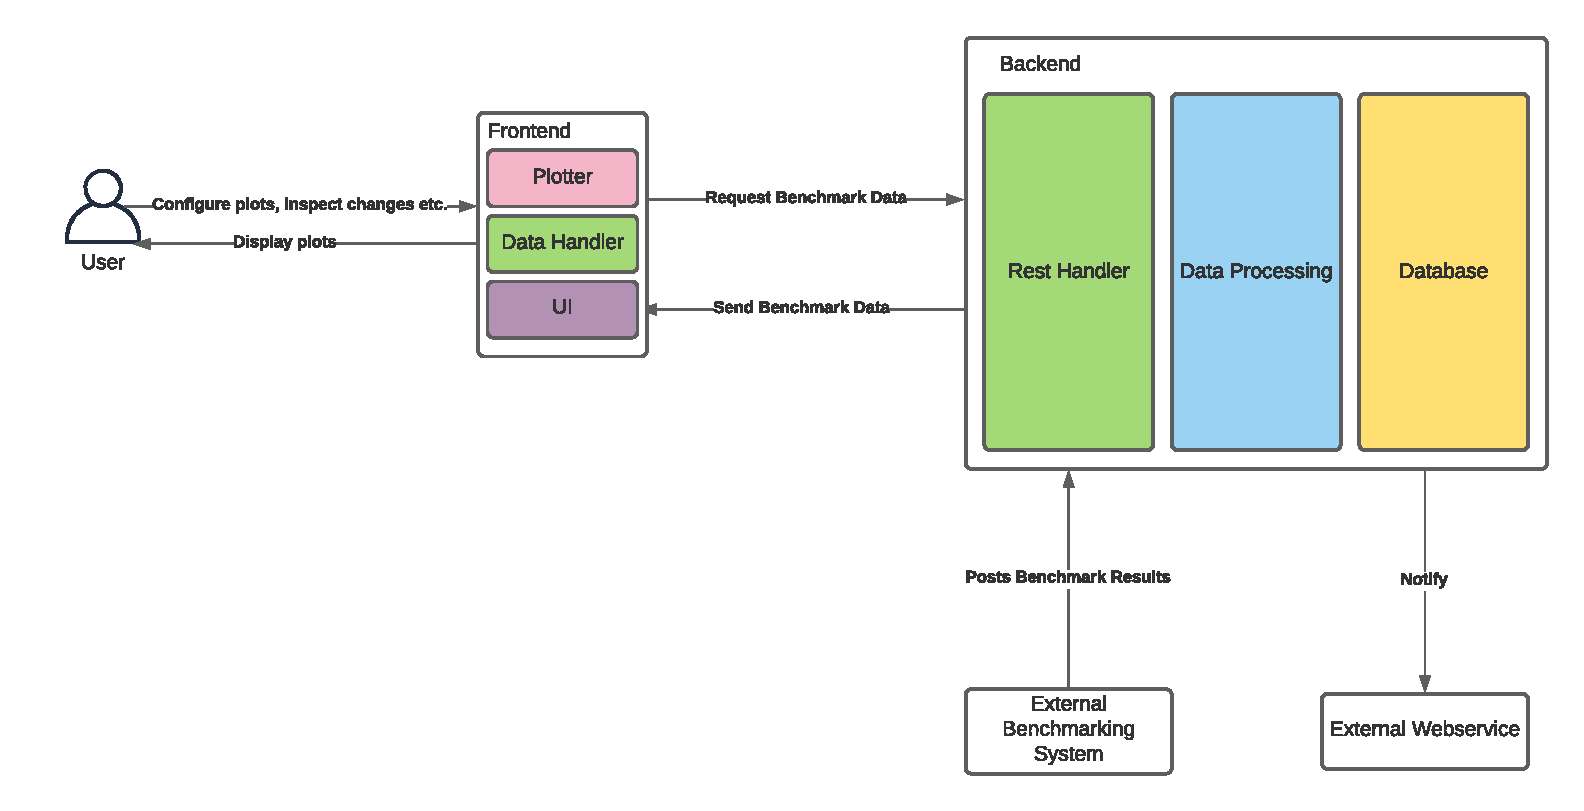
\includegraphics[width=\textwidth]{systemmodel.pdf}
    \caption{Diagram of system model}
    \label{fig:systemmodel}
\end{figure}

The system is split into frontend and backend. The \gls{user} only interacts with the frontend while any external systems like a benchmarking system or external webservices only interact with the backend. The frontend is realized through a web app.

\subsection{Frontend}

\subsubsection*{Plotter}

The Plotter is responsible for the generation of \gls{plot} from a given \gls{configuration} and benchmark results. 

\subsubsection*{Data Handler}

The Data Handler is responsible for requesting and receiving data from the backend. It does this by using the \gls{REST API} that is provided by the backend.

\subsubsection*{UI}

The UI handles interactions with the \gls{user} such as the creation of \glspl{configuration}.

\subsection{Backend}

\subsubsection*{REST Handler}

The Rest Handler provides the \gls{REST API} that gets consumed by the frontend and any external actors.

\subsubsection*{Data Processor}

The Data Processor is responsible for transforming the data and computing any metrics that might be needed.

\subsubsection*{Database}

The Database provides persistent storage for the Benchmark Data. It also provides interfaces retrieving the stored data.
